\documentclass[12pt]{report}

\usepackage[T1]{fontenc}
\usepackage[utf8]{inputenc}
\usepackage[italian]{babel}

\usepackage{mathtools}
\usepackage[]{float}
\usepackage{graphicx}
\usepackage{amsfonts}
\usepackage{amsthm}
\usepackage{amsmath}
\usepackage{amssymb}
\usepackage{makeidx}
\makeindex


\usepackage[a4paper, top=2.5cm, bottom=2cm, left=2cm, right=2cm]{geometry}

\usepackage[colorlinks=true, allcolors = black]{hyperref}

\swapnumbers
\theoremstyle{remark}
\newtheorem*{oss}{Oss}
\newtheorem*{nb}{N.B}
\newtheorem*{coro}{Corollario}
\newtheorem*{lemma}{Lemma}
\newtheoremstyle{theorem}
{10pt}
{0pt}
{}
{}
{\bfseries}
{\newline}
{10pt}
{}
\theoremstyle{theorem}
\newtheorem*{teo}{Teorema}
\newtheorem*{Def}{Def}


\begin{document}
	\date{}
	\author{Marco Militello}
	\title{Laboatorio II: Statistica e probabilità}
	\maketitle
	\tableofcontents
	\newpage

\chapter{Probabilità}
\index{Popolazione} \index{Evento casuale} \index{Variabile casuale} \index{Spazio campionario} \index{Campione} \index{Sample-space} \index{Teorema! Assiomi di Kolmogorov} \index{Probabilità! Classica} \index{Probabilità! Frequentista} \index{Teorema! Legge dei grandi numeri di Bernoulli} \index{Eventi indipendenti} \index{Probabilità condizionata} \index{Eventi indipendenti} \index{Teorema! Bayes} \index{Variabile aleatoria} \index{Random variable continua}

\section[Definizioni e teoremi]{Probabilità: definizioni e teoremi}
\begin{Def}[Evento casuale] \label{ev_casuale} 
	Associazione di una o più modalità ad un fenomeno casuale; risultato esperimento non prevedibile con certezza
	\begin{itemize}
	\item Ripetibile
	\item  Diverse modalità mutualmente esclusive
	\item Singolarmente imprevedibili	
	\end{itemize}
\end{Def}
\begin{Def}[Variabile casuale]\label{var_casuale} 
	Una variabile casuale è un numero reale da associare a una modalità di un fenomeno
	\begin{itemize}
		\item può essere discreta o continua
		\item Può assumere un numero finito o infinito
	\end{itemize}
\end{Def}
\begin{Def}[Spazio campionario]\label{spazio} 
	Insieme delle possibili modalità di un evento
\end{Def}
\begin{Def}[Popolazione]\label{popolazione} 
	Insieme dei possibili eventi; si può avere accesso a tutta la popolazione oppure solo ad una parte limitata (astrazione)
\end{Def}
\begin{Def}[Campione]\label{campione}
	Insieme degli eventi casuali raccolti
\end{Def}
\begin{Def}[Sample-space]\label{space}
	Contiene tutti i possibili eventi; la probabilità associata è 1\newline
	Sottoinsieme $\rightarrow$ può contenere uno o più eventi; si usa notazione insiemistica
\end{Def}
\begin{teo}[Assiomi di Kolmogorov $\rightarrow$ definizione assiomatica probabilità]\label{p_assiomatica}
	Probabilità di una funzione
	\[P: \; \Omega\to [0,1]\]
	tale che:
	\begin{itemize}
		\item $p(A) \ge 0$
		\item $p(\Omega) = 1$
		\item $p(A\cup B)=p(A)+p(B)$ se $A\cap B = \emptyset$ ($A$ e $B$ disgiunti) $\to$ eventi mutualmente esclusivi  
	\end{itemize}	
	Proprietà:
	\begin{itemize}
		\item $p(A) = 1- p(A^c)$ con $A^c$ evento complementare
		\item $p(A) \le 1$ con $p(A) = 1 \Rightarrow A $ evento certo e $p(A)=0 \Rightarrow A$ evento impossibile
		\item $p(\emptyset)=0$
		\item $B \subset A \Rightarrow p(A) \ge p(B)$
		\item $p(A\cup B) = p(A)+p(B)-p(A\cap B)$
	\end{itemize}
\end{teo}

\begin{Def}[probabilità classica]\label{p_classica}
	Rapporto casi favorevoli su casi possibili se i  casi sono ugualmente probabili
\end{Def}
\begin{Def}[probabilità frequentista]\label{p_frequentista}
	\[p(A)\sim \lim_{n\to\infty} \frac{n(A)}{N} \qquad N \text{ campione elementi, } n(A) \text{ numero successi}\]
\end{Def}
\begin{teo}[Bernoulli, legge dei grandi numeri]\label{teo:bernoulli}
	\[\lim_{N\to\infty} \frac{n(A)}{N} = p(A)\]
	Al crescere del numero di prove la frequenza relativa di 
	qualunque evento converge alla probabilità dell'evento
	\begin{itemize}
		\item Statistica frequentista $\to$ approccio limitante: associa probabilità all'accadare di un evento
		\item Approccio Bayesiano $\to$ Concetto plausibilità di un evento; conoscenza a priori: informazioni a priori
	\end{itemize}
\end{teo}

\begin{Def}[Probabilità condizionata]
	Nuova funzione di probabilità \qquad
	$P: \; \Omega \to [0,1], \; \text{A e B non disgiunti tra loro}$
	\[P(B|A) = {\frac{P(A \cap B)}{P(A)}} \qquad \text{B: varibile indipendente; A: parametro}\]
	Probabilità che si verifichi B sapendo che si è verificato A
\end{Def}

\begin{Def}[Eventi indipendenti]
	N eventi sono statisticamente indipendenti se la probabilità di un evento non è influenzata da uno o più eventi già verificati
	\begin{gather*}
		p(A \cap B) = p(A)\cdot  p(B) \\
		p(B|A) = p(B|\Omega) = p(B) \text{ e } p(A|B) = p(A|\Omega)=p(A) \Rightarrow \text{ statisticamente indipendenti}
	\end{gather*}	
\end{Def}

\begin{teo}[Bayes]
	\begin{gather*}
		p(A|B) = \frac{p(B|A)}{p(B)} \cdot p(A) \to p(\text{teoria}\, |\, \text{risultato}) 
		= \frac{p(\text{risultato}\, | \, \text{teoria})}{p(\text{risultato})} \cdot p(\text{teroria})\\
		p(A_j | E) = \frac{p(A_j)\cdot p(E|A_j)}{\sum_j [p(A_j)\cdot p(E|A_j)]} \qquad \text{$A_j$ mutualmente esclusivi}
	\end{gather*}
\end{teo}

\begin{Def}[Variabile aleatoria]
	Numero associato all'evento \newline
	$P: \, \Omega \to [0,1]$
	\begin{itemize}
		\item Sample-space sottoinsieme di $\mathbb{N}$ \qquad $p(k) > 0 \; \forall k$
		\item $p(k) = $probabilità valore k \qquad $\sum P_k = 1$
	\end{itemize}
\end{Def}

\begin{Def}[Random variable continua]
	evento identificabile con numero reale x a cui viene associata una densità di probabilità
	\[p(a<x<b) \qquad \text{intervallo} (a,b)\]
	\begin{itemize}
		\item il sample-space è $\Omega$ è un sottoinsieme di $\mathbb{R} \to \Omega \subseteq \mathbb{R}$
		\item la probabilità di uno specifico valore è infinitesima $\Rightarrow p(x) = 0 \; (\Omega \text{ contiene infiniti elementi})$
		\item la probabilità che viene associata a un gruppo di $\Omega$ 
	\end{itemize}
	Rappresentazione $\to$ ISTOGRAMMA (classi di frequenza $f = \frac{n}{N})$
	\begin{itemize}
		\item L'area di un bin è la probabilità che misura cada in quel bin
		\item integrale istogramma è 1
		\item il bin-size può essere ridotto $\to$ se il bin-size diventa infinitesimo $\Rightarrow$ distibuzione continua pdf
	\end{itemize}
\end{Def}

\chapter{Statistica}
\index{Densità di probabilità} \index{Densità di probabilità cumulativa} \index{Valore di aspettazione} \index{Media} \index{Varianza} \index{Mediana} \index{Moda} \index{Momenti}

\begin{Def}[Densità di probabilità]
	funzione pdf: $\Omega \subseteq \mathbb{R} \to \mathbb{R}^+$ ( non è una probabilità, ma una densità di probabilità)
	\[P(a<x<b) = \int_{a}^{b} pdf(x) \, dx \le 1\]
	\begin{itemize}
		\item $pdf(x)>0 \; \forall x$
		\item $\int_\Omega pdf(x) \, dx = 1$
		\item $P(a<x<b) = \int_a^b pdf(x) \, dx$
	\end{itemize}
\end{Def}

\begin{Def}[Densità di probabilità cumulativa]
	\' E una probabilità e indica la probabilità del punto x
	\[cdf = \int_a^x pdf(x) \, dx\]
	cdf è la primitiva della pdf $\to pdf(x) = \frac{d}{dx} cdf(x)$
\end{Def}

\begin{Def}[Valore di aspettazione]
	Media della funzione usando come peso la $pdf(x)$
	\[E(u(x))= \int_\Omega u(x)\cdot pdf(x)\, dx\]
	\begin{itemize}
		\item $E(u(x)+v(x)) = E(u(x))+E(v(x))$
		\item $E(k\cdot v(x)) = k\cdot E(u(x))$
	\end{itemize}
\end{Def}

\section{Stime di tendenza centrale}
\subsection{Media aritmetica}
\begin{Def}[Media $\mu$]
	Valore di aspettazione di $x$ 
	\[E(x) = \int x\cdot pdf(x) \, dx = \mu\]
	\begin{enumerate}
		\item Somma scarti della media è nulla
		\item $\overline{x}$ rende minima $\displaystyle \sum_{i=1}^N {(x_i-x)}^2$
		\item media $\mu \neq$ media campionaria $\left(\displaystyle\overline{x} = \frac{1}{N} \sum_{i=1}^N x_i\right)$
  \item La media aritmetica di un insieme di dati numerici è quel valore che rende minima la somma dei quadrati degli scarti dalle $x_i$
	\end{enumerate}
La media aritmetica è la stima migliore, ha un errore inferiore di quello delle misure stesse
\end{Def}

\subsection{Moda}
\begin{Def}[Moda]
	Tendenza centrale del campione; massimo della pdf: può essere più di uno $\to$ valore che si è presentato più volte
	\begin{itemize}
		\item Distribuzioni amodali (no massimo)
		\item Distibuzioni multimodali (più massimi)
	\end{itemize}
Talvolta si dice che la distribuzione non ha moda anche se presenta un massimo, quando quest'ultimo si trova in uno degli estremi dell'intervallo che contiene le misure 	
\end{Def}

\subsection{Mediana}
\begin{Def}[Mediana]
	Punto che divide area pdf(x) in due metà: è il valore centrale se il numero di misure è dispari, altrimenti è la semisomma dei valori centrali; la mediana esiste sempre
\end{Def}
Media, moda e mediana sono stime di tendenza centrale 

\section{Momenti}
	\begin{description}
		\item [Momento di ordine m] della pdf $\to$ valore di aspettazione di $x^m$ 
		\item \[E(x^m) = \int x^m \cdot pdf(x) \, dx\]
		\begin{itemize}
			\item momento di ordine 1 $\to$ media
		\end{itemize}
		\item [Momenti centrali di ordine m] della pdf $\to$ valore di aspettazione di ${(x-\mu)}^m$
		\begin{itemize}
			\item momento centrale di ordine 1 $\to E(x-\mu) =0$
			\item momento centrale di ordine 2 $\to$ Varianza o scarto quadratico medio $\sigma^2$ \newline
				Valore di aspettazione di ${(x-\mu)}^2$
				\[E({(x-\mu)}^2) = \int {(x-\mu)}^2 \cdot pdf(x) \, dx = \sigma^2\]
				$\sigma =$ deviazione standard ed è legato alla larghezza della pdf(x)
				\begin{gather*}
					\sigma^2 = E(x^2)-\mu \\
					\sigma^2 = \frac{1}{N} \sum_{i=1}^{N}{(x_i-x)}^2 = \frac{1}{N}x_i^2-\bar{x}^2
				\end{gather*}	
			\item momento centrale di ordine 3 $\to$ legato a parametro SKEWNESS (misura asimmetria curva)
			\[\gamma_1 = \frac{E({(x-\mu)}^3)}{\sigma^3}\qquad \begin{cases}
				\gamma_1 = 0 \; &\text{simmetrica}\\
				\gamma_1 <0 \; &\text{destra}\\
				\gamma_1 >0 \, &\text{sinistra}
			\end{cases}\]
			\item momento centrale di ordine 4 $\to$ legato a parametro KURTOSI (misura quanto è piccata la curva)
			\[\gamma_2 = \frac{E({(x-\mu)}^4)}{\sigma^4} -3 \qquad \begin{cases}
				\gamma_2= 0 \; & \text{gaussiana} \\
				\gamma_2>0 \; &\text{+ piccata}\\
				\gamma_2<0 \; &\text{- piccata}
			\end{cases}\]			
		\end{itemize}
	\end{description}


\noindent Se esistono tutti i momenti centrali $\Rightarrow$ caratterizzano in modo univoco la pdf; se due variabili casuali hanno stessi momenti fino a qualsiasi ordine, allora la loro densità di probabilità è identica

\begin{Def}[Riproduttività]
	Siano x,y random variable distribuite secondo stessa pdf; se $z=x+y$ (z random variable) ha la stessa pdf $\Rightarrow$ pdf gode della proprietà riproduttiva
\end{Def}

\noindent La $pdf(x;\alpha_1,\alpha_2,\dots)$ è caratterizzata da:
\begin{itemize}
	\item una forma funzionale 
	\item uno o più parametri
\end{itemize} 

\section{Distibuzioni}
\subsection*{Distribuzione gaussiana}
\[pdf(x;\mu,\sigma) = \frac{1}{\sqrt[]{2\pi}\sigma} e^{-\frac{{(x-\mu)}^2}{2\sigma^2}}\]
Gode della proprietà riproduttiva \newline
FWHM(largezza a mezza altezza) $\sim 2.35\sigma$ \newline
Distribuzione gaussiana standardizzata  $\to \mu=0 \; \sigma=1$
\[G(x) = \frac{1}{\sqrt[]{2\pi}}e^{-\frac{x^2}{2}}\]
\[cdf(x) = \int_{-\infty}^x G(x) \to erf(x) = \frac{1}{\sqrt[]{2\pi}} \int_{-\infty}^x e^{-\frac{x^2}{2}}\]
$erf(x)$ non ha una definizione univoca
\begin{itemize}
	\item media: \; $E(x)=\mu$
	\item varianza: \; $Var(x)=\sigma^2$
	\item skewness: \; $\gamma_1=0$
	\item kurtosi: \; $\gamma_2=0$
\end{itemize}

\noindent Le misure affette da errori casuali hanno una probabilità del 68\% di cadere all'interno di un intervallo di semiampiezza $\sigma$ centrato sul valore vero della grandezza; l'intervallo ha quindi il 68\% di probabilità di contenere il valore vero (se gli errori sono casuali e normali) \newline
L'errore quadratico medio $\sigma$ può essere interpretato come valore assoluto delle ascisse dei due punti di flesso della Gaussiana 

\begin{figure}[H]
    \centering
    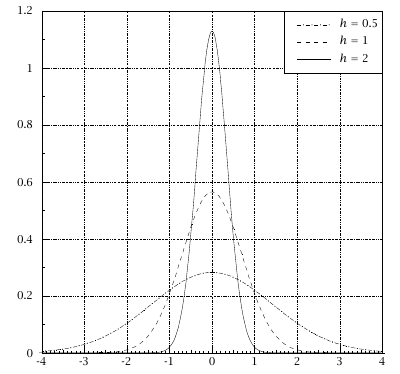
\includegraphics[width=10cm]{immagini/gauss.png}
    \label{fig:gauss}
\end{figure}

\subsection*{Distribuzione Breit-Wigner (o Cauchy)}
\[BW(x;\alpha,M) = \frac{1}{\pi\alpha}\frac{1}{1+\frac{{(x-M)}^2}{\alpha^2}}\]
es: fisica nucleare \newline
Nessuno dei momenti centrali esistono, nemmeno la media; M è la mediana della distribuzione e $\alpha$ è la larghezza a metà altezza \newline
Il valor medio di un campione proveniente da una popolazione che segua distribuzione di Cauchy è distribuito anch'esso secondo Cauchy

\begin{figure}[H]
    \centering
    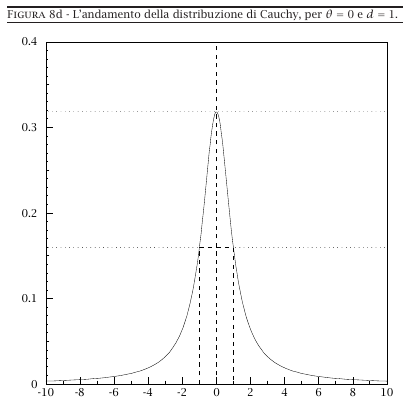
\includegraphics[width=10cm]{immagini/breit-wigner.png}
    \label{fig:breit}
\end{figure}

\begin{Def}
	Rappresentazione con distribuzione di probabilità; si estrae un campione dalla popolazione	
\end{Def}

\subsection*{Campionamento di una $pdf(x)$}
\begin{itemize}
	\item gli eventi che formano il campione sono numeri relativa
	\item la popolazione è completamente rappresentata dalla $pdf(x)$
	\item l'operazione di campionamento della pdf consiste nell'estarre numeri che siano rappresentativi della pdf stessa
\end{itemize}

\begin{teo}[del limite centrale]
	Il teorema stidia la pdf di una r.v. costruita in modo analogo $pdf_1(\mu_1,\sigma_1),\dots, pdf_N(\mu_N,\sigma_N)$ 
	\begin{itemize}
		\item consideriamo N variabili aleatorie indipendenti $x_i$, ciascuna caretterizzata da $pdf_i$
		\item assummiamo che per ogni $pdf_i$ esistano finite media $\mu_i$ e varianza $\sigma_i$
		\item definiamo nuova random variable $\bar{x}$ costruita come media aritmetica delle r.v. di ciascuna $pdf_i$
		\[\bar{x} = \sum_{i=1}^N \frac{x_i}{N}\]
		\end{itemize}
	Allora se $N\to\infty$$\bar{x}$ è distibuita in modo gaussiano con media pari alla somma delle medie e varianza pari alla somma delle varianze (media pari a $\mu$ e varianza pari a $\frac{\sigma^2}{N}$)
	\begin{gather*}
		E[\bar{x}] = \mu_{\bar{x}} = \sum_{i=1}^N \frac{\mu_i}{N}\\
		Var[\bar{x}] = \sigma^2_{\bar{x}} = \sum_{i=1}^N \frac{\sigma^2_i}{N^2}\\
		pdf \left(\sum_{i=1}^N \frac{x_i}{N}\right) \to Gauss(\mu_{\bar{x}},\sigma_{\bar{x}}) \quad N\to\infty
	\end{gather*}
\end{teo}

\subsection*{Misura come variabile aleatoria}
Misura come grandezza fisica $\to$ affetta da errore casuale
\begin{itemize}
	\item $x_0:$ valore vero della grandezza che misuriamo
	\item $x:$ risultato della singola misura
	\item $\varepsilon = \sum \varepsilon_i:$ errore associato ad ogni misura $\to$ somma dei $\varepsilon_i$ casuali
\end{itemize}
Allora
\[x = x_0 + \varepsilon\]
x è una variabile aleatoria associata a $pdf(x)$ \newline
Ripetere misura equivale a campionare la pdf(x), che dipende da $pdf(\varepsilon)$ \newline
Se $\varepsilon = \sum \varepsilon_i$ sono casuali $\Rightarrow pdf(\varepsilon)$ è una gaussiana centrata in 0; se non è centrata in 0 allora sono presenti degli errori sistematici

\subsection*{Cambio di variabili nelle pdf}
x è una r.v. descritta da $pdf_1(x) \to y=y(x) \Rightarrow pdf_2(y)$ con $y$ biunivoca, monotona e derivabile
\begin{enumerate}
	\item Calcolo $pdf_2(y)$ in forma analitica
	\item determino $\mu_y \; \sigma_y$ della $pdf_2(y)$ con la propagazione degli errori
\end{enumerate}

\[pdf_2(y) = pdf_1(x) \cdot |x'(y)| = odf_1(x) \cdot \frac{1}{|y'(x)|} = pdf_1(x(y))\cdot |x'(y)|\]
\[pdf_2(x) = pdf_1(x) \cdot \left| \frac{dx}{dy} \right|\]

\subsection*{Distribuzione lognormale}
x r.v. con distribuzione gaussiana \newline
$y=e^x \Rightarrow x=\log{y} \; x' = \frac{1}{y}$
\[pdf(y;\mu,\sigma) = \frac{1}{\sigma \sqrt[]{2\pi}} e^{-\frac{{(\log{y}-\mu)}^2}{2\sigma^2}}\]

\begin{gather*}
	E[x] = e^{\left(\mu + \frac{\sigma^2}{2}\right)}\\
	E[x^2] = e^{(2\mu + 2\sigma^2)} \\
	Var[x] = e^{(2\mu + 2\sigma^2)}\left(e^{\sigma^2}-1\right)
\end{gather*}

\begin{figure}[H]
    \centering
    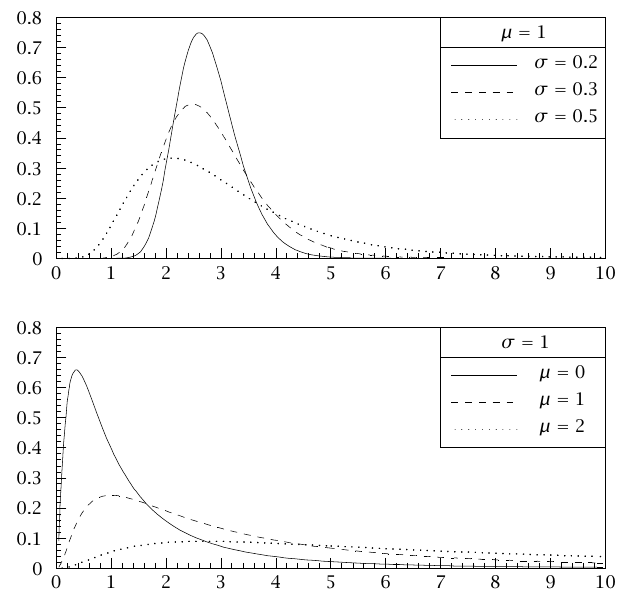
\includegraphics[width=10cm]{immagini/log-normale.png}
    \label{fig:log-normale}
\end{figure}

\section{Propagazione degli errori}

\begin{itemize}
	\item $y = ax +b$ \; Lineare \quad $\mu_y = a\mu_x +b \qquad \sigma^2_y = a^2\sigma^2_x$ \; Formula esatta di propagazione degli errori 
	\item $y=y(x)$ \; non lineare \qquad y(x) = y($\mu_x$) + $\frac{dy}{dx}\Big|_{\mu_x}(x-\mu_x$)+ $\dots$ \; Taylor 
	\[y(\mu_x) = \int (x-\mu_x)\cdot pdf(x) \, dx \quad\text{ approssimazione primo ordine}\]
	\[\mu_y \simeq y(\mu_y)+\frac{1}{2} \frac{d^2y}{dx^2}\Big|_{\mu_x}\sigma^2_x \qquad \sigma^2_y \simeq {\left(\frac{dy}{dx}\Big|_{\mu_x}\right)}^2\sigma^2_x \quad \text{ approssimazione secondo ordine}\]
\end{itemize}
Questa si chiama formula approssimata di propagazione degli errori; per essere applicata gli errori non devono essere troppo grandi e le variabili stesse devono essere tra loro statisticamente indipendenti \newline
Se l'evento casuale è identificabile con un numero intero k $\Rightarrow$ r.v. discreta:

\begin{itemize}
	\item il sample-space $\Omega$ è un sottoinsieme di $\mathbb{N}$
	\item $P(k) =$ probabilità che r.v. assuma valore k
	\item $P:\, (\Omega \subseteq \mathbb{N}) \mapsto [0,1]$
\end{itemize}

\noindent Allora gli assiomi di Kolmogorov diventano:

\begin{itemize}
	\item $P(k)>0 \, \forall k$
	\item $\sum_{\forall k\in \Omega} P(k) = 1$
	\item $P(k\, \&\, h) = P(k) + P(h) \quad \forall k,n \in \Omega \; h \neq k$
\end{itemize}

\subsection*{Bernoulli trial o distribuzione binomiale}
Identifica la probabilità che un evento k si verifichi esattamente N volte, con ognuna delle prove statisticamente indipendente dalle altre
Distribuzione Binomiale: discrive k successi in N prove

\[B(k,N,p) = \binom{N}{k} p^k {(1-p)^{N-k}}\]

\begin{description}
	\item[media:] \; $\mu = \displaystyle \sum_{k=0}^N k\cdot B(k,N,p) = Np$
	\item[varianza:] \; $\sigma^2 = Var[k] = Np(1-p)$ 
\end{description}
\noindent Quando il numero di prove N è sufficientemente elevato e la probabilità p non è troppo vicina ai valori estremi di 0 e 1, allora di distribuzione binomiale è ben approssimata da una distribuzione binomiale; in generale si ritiene che l'approssimazione sia accettabile quando entrambi i prodotti Np e Nq hanno valore inferiore a 5 \newline
Vale proprietà riproduttività

\[\gamma_1 = 
\begin{cases}
	\frac{1-2p}{\sqrt[]{N_p(1-p)}} & p \neq 0\\
	0 & p= {\frac{1}{2}}	
\end{cases}\quad \gamma_1 \to 0\; N\to \infty\]

\[\gamma_2 = \frac{1-6p(1-p)}{N} \quad \gamma_2 \to 0 \; N\to\infty\]

\noindent Se $N\to\infty$ Binomiale asintotica ad una Gaussiana: $ \; B(k;N,p) \simeq G(k;\mu,\sqrt[]{\mu})$ \newline
Se $p\to 0$ e $N\cdot p$ è finito $\Rightarrow$ Binomiale asintotica a Poissoni: \; $B(k;N,p) \simeq P(k;\lambda) \; \lambda=N\cdot p$

\subsection*{Distibuzione di Poisson}
\begin{itemize}
	\item La probabilità del verificarsi di un evento in un intervallo di tempo molto piccolo dt è proporzionale alla durata di tale intervallo 
 \item Il verificarsi o meno di un evento in uncerto intervallo di tempo è indipendente dal verificarsi o meno di un evento prima o dopo di esso 
\end{itemize}
Probabilità di contare k eventi in un intervallo $\Delta x$ unitario; è il caso di un processo per cui la frequenza media è $\lambda$ costante \newline
L'accadere di un evento è indipendete dall'accadere di un evento successivo

\[Poiss(k;\lambda) =  \frac{e^{-\lambda}}{k!}\lambda^k \qquad k\in [0,\infty) \quad \lambda=\frac{E[k]}{\Delta x=1} \text{ media pdf}\]

\begin{itemize}
	\item probabilità evento dx è proporzionale all'ampiezza dell'intervallo $p\cdot dx$
 \item p costante indipendente da x: FREQUENZA MEDIA COSTANTE 	
 \item la probabilità di avere più di un evento in dx è nulla: EVENTI PARI
 \item eventi indipendeti tra loro 
\end{itemize}
\begin{itemize}
	\item [*] $p(1 \text{ evento in } dx) = p\cdot dx$
 \item [*] $p(0 \text{ eventi in }dx) = 1 -p\cdot dx$
 \item [*] $p(0 \text{ eventi in } [0,x]) = q(x)$
 \item [*] $p(0 \text{ eventi in } [0,x+dx]) = q(0,x+dx)$
\end{itemize}
\begin{gather*}
	q(x+dx) = q(x)(1-pdx) \\
	\frac{q(x+dx)-q(x)}{dx} = -p\cdot q(x) \\
	q(x) = q(0)e^{-px} \qquad q(0)\text{ da normalizzazione pdf: } \int_\Omega q(x) = 1
\end{gather*}
La probabilità di non avere eventi in $[0,x]$ è data da esponenziale; la probabilità di avere 0 eventi in $[0,x_1]$ e 1 eventi in $[x_1,x_1+dx]$ è uguale a $e^{-px_1}(pdx_1)$ \newline
Probabilità di avere k eventi in $[0,x]: \; e^{-px}\frac{{(px)}^k}{k!}$
\begin{description}
	\item[Media:] \; $\mu = E[k]= \displaystyle \sum_{k=0}^\infty k\cdot Poiss(k;\lambda) = \lambda$
 \item[Varianza] \; $\sigma^2 = \lambda=x$
 \item[] $\gamma_1 = \frac{1}{\sqrt[]{x}} \qquad \gamma_2 = \frac{1}{\lambda}$
\end{description}
Se $\lambda \to \infty \Rightarrow$ Poiss$(k;\lambda) \to$ Gauss$(k;\lambda,\sqrt[]{\lambda})$ \newline
La distribuzione di Poisson è una approssimazione alla distribuzione binomiale che si può ritenere valida qualora si verifichino eventi casuali di probabilità estremamente piccola, e che ci è possibile vedere solo quando si compiono osservazioni su un numero elevato di esistano
\[p^2 << p \qquad p<<Np<<N\]

\begin{figure}[H]
    \centering
    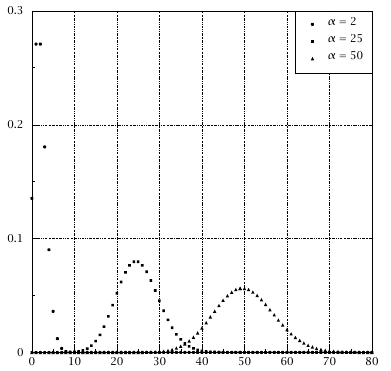
\includegraphics[width=0.5\textwidth]{immagini/poisson.png}
    \label{fig:poisson}
\end{figure}

\subsection*{Distribuzione esponenziale}
\[pdf(t) = \frac{1}{\tau}e^{-\frac{t}{\tau}}\qquad p=\frac{1}{\tau}\]
\begin{description}
	\item[Media:] $\tau$
 \item[Varianza:] $\tau^2$  
\end{description}

\section{PDF IN N-DIMENSIONI}
Un evento può essere identificato da un vettore $\to$ valgono gli assiomi di Kolmogorov 
\begin{gather*}
	pdf(\vec{x}): \, \mathbb{R}^n \to \mathbb{R}^+ \\
	cdf(\vec{x}): \, \int_{-\infty}^{\vec{x}} pdf(\vec{x})\, d\vec{x}
\end{gather*}
\begin{description}
	\item[Media:] $\vec{\mu} = \left(
		\begin{array}{c}
			\mu_1 \\
			\vdots \\
			\mu_N
		\end{array} \right) = E[\vec{x}] = \int \vec{x}pdf(\vec{x})d\vec{x} \quad E[x_i] = \int x_ipdf(\vec{x})d\vec{x}$
	\item[Varianza:] matrice di covarianza $n\times n \quad \sigma^2_{ij} = [(x_i-\mu_i)(x_j-\mu_j)]$
\end{description}
pdf congiunta tra r.v $\{x_1,\dots, x_N\} \; pdf(\vec{x}) \leftrightarrow pdf(x_1, \dots, x_N)$ \newline
$pdf_n(x)$ marginale $\to$ distribuzione di x indipendente da y
\[pdf_n(x) = \int pdf(x,y)\, dy\]
Probabilità condizionata: $pdf(x\,|\, y=y_0) \to pdf$ associata ad x quando $y=y_0$
\[pdf(x\,|\, y=y_0) = \frac{pdf(x,y_0)}{pdf_{ny}(y_0)} \quad pdf_{ny}(y_0)\text{ normalizzazione}\]
x e y sono indipendenti $\iff pdf(x,y) = pdf_{nx}(x)\cdot pdf_{n_y}(y)$ 
\begin{gather*}
	E[\mu(x,y)] = \iint \mu(x,y)pdf(x,y) \, dx\,dy \\
	\mu_x= E[x] = \int x\,dx \int pdf(x,y) \, dy \\
	Var[x] = E[{(x-\mu_x)}^2] = \sigma^2_x \\
	Cov[x,y] = E[(x-\mu_x)(y-\mu_y)] = E[(x,y)]\mu_x\mu_y
\end{gather*}
\begin{itemize}
	\item x e y sono indipendenti $\Rightarrow Cov[x,y] = 0$, ma $Cov[x,y]=0$ non implica x e y indipendenti
 \item x e y legati linearmente $\Rightarrow Cov[x,y] =0$
\end{itemize}
\subsection{Matrice covarianza}
La matrice V di covarianza è simmetrica \newline
Coefficiente di correlazione 
\[\rho_{xy} = \frac{Cov[x,y]}{\sigma_x\sigma_y} \quad \rho^2 \le 1\]
$\rho^2 =0$ se x e y sono legati linearmente \newline
Il coefficiente di correlazione è ovviamente adimensionale ed è nullo quando le variabili stesse sono statisticamente indipendenti; il suo valore è compreso tra -1 e 1 
\begin{teo}
	Due differenti combinazioni lineari delle stesse variabili sono sempre correlate \newline
\end{teo}
\noindent Cambio di variabili per rendere covarianza nulla $\Rightarrow$ variabili non correlate, ma non indipendenti
\begin{gather*}
	\vec{x} \mapsto \vec{y} = f(\vec{x})\\
	pdf_x(\vec{x}) \mapsto pdf_y(\vec{y})
\end{gather*}
Caso bidimensionale $\rightarrow pdf_x(x_1,x_2):$ pdf congiunta
\[\begin{cases}
	x_1 \to y_1=v_1(x_1,x_2)\\
	x_2\to y_1=v_2(x_1,x_2)
\end{cases}\]
\[pdf(y_1,y_2)dy_1dy_2 = pfd(x_1,x_2)dx_1dx_2\]
Funzioni inverse
\[\begin{cases}
	x_1=w_1(y_1,y_2)\\
	x_2=w_2(y_1,y_2)
\end{cases}\]
In generale
\[pdf_y(y_1,y_2) = pdf_x(w_1(y_1,y_2),w_2(y_1,y_2))\det J \qquad \text{J: Jacobiano}\]
Le trasformazioni di variabili si usano per:
\begin{itemize}
	\item ridefinire le variabili in modo che Cov[x,y]=0
 \item Generare numeri casuali: Box-Muller
\end{itemize}
\subsection{Propagazione degli errori per variabili correlate}
\[F = F(x_1, \dots , x_N )\]
Introduco vettore F di dimensione N con componenti
\[F_i = \frac{\delta F}{\delta x_i}\]
e il suo trasposto $F^T$ \newline
Allora 
\[Var(F) = F^T V F\]

\subsection{Pdf normale multivariata}
Estensione n-dimensionale della Gaussiana
\[E[\vec{x}]=\int \vec{x}pdf(\vec{x})\,d\vec{x}\]
Matrice di covarianza	
\[\Sigma = E[(x_i-\mu_i)(x_j-\mu_j)] = \sigma^2_{ij} = Cov[x_i,x_j]\]
\[N(\vec{x};\vec{\mu},\Sigma) = \frac{1}{\sqrt[]{{(2\pi)}^n\det (\Sigma)}}e^{(-\frac{1}{2}{(\vec{x}-\vec{\mu})}^T \Sigma^{-1}(\vec{x}-\vec{\mu}))}\]
In 2 dimensioni:
\[\Sigma = \left(\begin{array}{cc}
	\sigma^2_x & \rho\sigma_x\sigma_y \\
	\rho\sigma_x\sigma_y & \sigma^2_y
\end{array}\right)\]
\[N(\vec{x};\vec{\mu},\Sigma) = \frac{1}{\sqrt[]{{(2\pi)}^2\sigma^2_x\sigma^2_y(1-\rho)}}e^{-\left(\frac{1}{2(1-\rho^2)}\left[{\left(\frac{x-\mu_x}{\sigma_x}\right)}^2-2\rho\left(\frac{x-\mu_x}{\sigma_x}\right)\left(\frac{y-\mu_y}{\sigma_y}\right)+{\left(\frac{y-\mu_y}{\sigma_y}\right)}^2\right]\right)}\]
$-\frac{1}{2(1-\rho^2)}\left[{\left(\frac{x-\mu_x}{\sigma_x}\right)}^2-2\rho\left(\frac{x-\mu_x}{\sigma_x}\right)\left(\frac{y-\mu_y}{\sigma_y}\right)+{\left(\frac{y-\mu_y}{\sigma_y}\right)}^2\right]
=k=cost \to$ Curve di equiprobabilità

\subsection{Binomiale standardizzata}
$\vec{\mu}=0 \; \sigma_x=\sigma_y=1$ \newline
Media e moda coincidono \newline
Massimo per k=0 $\to$ origine
\[N(\vec{x}) = \frac{e^{-\left(-\frac{1}{2(1-\rho^2)}(x^2-2\rho xy +y^2)\right)}}{2\pi \sqrt[]{1-\rho}}\]
Curve di equiprobabilità: ellissi centrati nell'origine \newline
Forma a campionaria
\begin{itemize}
	\item $\rho=0 \to$ cerchi
 \item $\rho\to 1 \Rightarrow$ ellisse degenera nella retta 
\end{itemize}
$k = -\frac{1}{2} \to$ riduce densità di $\frac{1}{\sqrt[]{e}}$ rispetto al massimo \newline
Ellisse degli errori $(\mu_x \pm \sigma_x; \mu_y \pm \sigma_y) \to $ inegrale pdf su questo ellisse $\Rightarrow 39\%$ \newline
La matrice di covarianza è diagonalizzabile $\Rightarrow$ Esiste cambio di variabili con variabili non correlate

\section{Stime parametri}
\begin{Def}[Statistica]
	Una statistica è una funzione che dato un campione restituisce le proprietà e i parametri; variabile aleatoria: funzione degli N campionamenti
\end{Def}
\begin{Def}[Stimatore]
	Uno stimatore è una statistica che usa N campionamenti per fornire una stima dei parametri; uno stimatore è dunque una funzione di variabili casuali e di conseguenza una variabile casuale 
	\[\bar{\theta} = \bar{\theta} = (x_1,x_2,\dots ,x_N)\]
\end{Def}
\begin{Def}[Stimatore consistente]
	Uno stimatore si dice consistente se converge probabilisticamente al valore vero del parametro
	\[\lim_{N\to\infty} \bar{\theta}(x_1,x_2,\dots , x_n) = \theta^*\]
\end{Def}
\begin{Def}[Stimatore unbiased]
	Uno stimatore si accurato (unbiased) se mediamente coincide con il valore vero del parametro
	\[E[\bar{\theta}] = \int \bar{\theta} pdf_{\bar{\theta}}(\bar{\theta}) \, d\bar{\theta} = \theta^*\]
	Il bias non è sempre valutabile a priori
	\[E[\bar{\theta}_N] - \theta^*\]
\end{Def}
\begin{Def}[Stimatore efficiente]
	Uno stimatore si dice tanto più efficiente tanto è minore la sua varianza; l'efficienza determina la precisione dello stimatore \newline
	\hyperref[teo:Rao]{Teorema di Rao-Cramer}
\end{Def}

\section{Funzione di verosimiglianza}
Dato un campione di N eventi indipendenti $x_i$ allora si può costruire una funzione di verosimiglianza che rappresenta la densità di probabilità da associare all'evento casuale consistente nell'essere un certo $\theta$ il valore vero del parametro
\[\mathcal{L} (x_1,x_2,\dots ,x_N; \theta) = \prod_{i=1}^N f(x_i;\theta) \] \label{likelihood}
in cui la variabile indipendente è $\theta$ e il gli $x_i$ sono costanti
Il metodo di massima verosimiglianza consiste nello stimare il parametro $\theta$ come il valore che rende massima la \hyperref[likelihood]{funzione di verosimiglianza}
\[\frac{d \mathcal{L}}{d\theta}=0 \qquad \frac{d^2\mathcal{L}}{d\theta^2}<0\]
Nel caso abbiano più soluzioni si sceglie il massimo assoluto \newline
Dato che il logaritmo naturale è una funzione monotona strettamente crescente allora il massimo della $\ln\mathcal{L}$ corrisponde al massimo della $\mathcal{L}$
\begin{enumerate}
	\item Lo stimatore di massima verosimiglianza è una stima asintoticamente consistente al crescere della dimensione del campione
 \item Lo stimatore di massima verosimiglianza ha una densità di probabilità asintoticamente normale al crescere della dimensione del campione
 \item Lo stimatore di massima verosimiglianza è asintoticamente anche lo stimatore più efficiente
 \item Asintoticamente gli stimatori della maximum likelihood sono efficienti e privi di bias 
\end{enumerate}
La funzione di verosimiglianza permette:
\begin{itemize}
	\item di misurare l'informazione dei campionamenti sul parametro; consente di studiare tecniche per ridurre i dati senza perdere informazioni
 \item  di valutare la minima varianza raggiungibile con uno stimatore
 \item di realizzare un metodo per costruire uno stimatore 
\end{itemize}

\begin{teo}[Rao-Cramer]\label{teo:Rao}
	Una qualsiasi stima imaparziale $\bar{\theta}$ del parametro ha una varianza che non può essere inferiore ad un valore limite
	\[Var(\bar{\theta}) \ge \frac{\left[1+\frac{\delta b_n}{\delta\theta}\right]}{E\left[-\frac{\delta^2 \ln(\mathcal{L}(\vec{x};\theta))}{\delta\theta^2}\right]}\] 
	Uno stimatore si dice efficiente se vale l'uguale nella relazione; in questo caso lo stimatore di minima varianza rende massima la funzione di verosimiglianza
\end{teo}

\section{Metodo dei minimi quadrati}
Abbiamo un modello che definisce relazione tra due grandezze fisiche X e Y; con metodo minimi quadrati cerchiamo parametri che rendono minima la distanza tra parametri e modello, a differenza del metodo della maximum likelihood che rende massima la probabilità, dato un modello, di osservare i nostri dati campionati
\[Q^2(\theta) = \sum_{i=1}^N \frac{{[y_i - f(\vec{\theta},x_i)]}^2}{\sigma^2_i}\]
$Q^2$ è la somma dei quadrati delle distanze tra i punti campionati e la funzione $Y = f(\vec{\theta}, X)$; ciascuna distanza è normalizzata alla larghezza della $pdf(y_i)$ \newline
Quando le $pdf_i(y_i)$ sono gaussiane i due stimatori (ML e LQ) coincidono 
\begin{teo}[di Gauss-Markov]
	Considero due grandezze fisiche X e Y legate da una relazione lineare nei parametri; i dati sono N misure $y_i$ del valore della granezza Y effettuate in corrispondeza di uno specifico valore $x_i$ della gandezza X. Non c'è errore sulle $x_i$ mentre le variabili $y_i$ sono variabili casuali indipendenti tra di loro. \newline
	Sotto queste ipotesi, nel caso di un modello lineare nei paramtrei, lo stimatore dei minimi quadrati è unbiased e, tra tutti gli stimatori unbiased e lineari nei parametri, è quello con varianza minima
\end{teo}

\section{Test del Chi-Quadro}
Nel caso di pdf gaussiane, il valore assunto dal funzionale nel minimo è usato per verificare la compatibilità dati-modello
\[\chi^2_{min} = \sum_{i=1}^N \frac{{(y_i-\mu_i)}^2}{\sigma^2_i}\]
Questa è l'espressione di un $\chi^2$ a N-K gradi di libertà \newline
Il test del $\chi^2$ è uno dei possibili test di ipotesi per validare o confutare la validità di un modello
\[\chi^2_{rid} \frac{\chi^2}{N-K} \sim 1\]
Si scegli un criterio per il rigetto delle ipotesi: quando il $\chi^2$ cade nella coda di destra della distribuzione di probabilità che corrisponde al 5\% 
\[\int_{\chi^2_{min}}^\infty pdf(\chi^2)\, d\chi^2 > 0.05\]
Il test del $\chi^2$ valuta la bontà del fit riassumendo il risultato in un singolo valore. Per analizzare in dettaglio quanto è buono o meno l'accordo tra modello e dati si posso studiare:
\begin{itemize}
	\item i residui
		\[res_i = y_i - f(x_i,\vec{\theta^*_{LS}})\]
		questi sono una r.v. distribuita in modo gaussiano attorno al valore medio nullo con deviazione standard $\sigma_i$
	\item i residui normalizzati 
		\[res_i = \frac{y_i - f(x_i,\vec{\theta^*_{LS}})}{\sigma_i}\]
		questi ssono una r.v. distribuita in modo gaussiano attorno ad un valore medio nullo con deviazione standard 1
\end{itemize}

\end{document}